\documentclass[10pt]{article}

\usepackage{verbatim}
\usepackage{calc}
\usepackage{epsfig}
\usepackage{url}
\usepackage{longtable}
\input{pstricks}
\usepackage{multirow}
\usepackage{epstopdf}
\usepackage{graphicx}
\usepackage{type1cm}
\usepackage{eso-pic}
\usepackage{color}
\usepackage{cite}
\usepackage{listings}

\graphicspath{ {../fig/} }

\setlength{\textwidth}{6in}
\setlength{\textheight}{9in}
\setlength{\oddsidemargin}{(\paperwidth-\textwidth)/2 - 1in}
\setlength{\topmargin}{(\paperheight-\textheight -\headheight-\headsep-\footskip)/2 - 1.2in }

% enable/disable WBS tables
\newif\ifwbs
\wbsfalse
%\wbstrue

% enable/disable margin comments
\newif\ifcomments
%\commentsfalse
\commentstrue

\newcommand{\ngrm}{NGRM}
\newcommand{\ngrmfull}{Next Generation Resource Manager}
\newcommand{\ngjs}{NGRM Job Scheduler}
%\newcommand{\zMQ}{${\varnothing}$MQ}
\newcommand{\zMQ}{\O{}MQ}
\newcommand{\slurm}{Slurm}
\newcommand{\moab}{Moab}
\newcommand{\openmpi}{OpenMPI}
\newcommand{\mpich}{MPICH}
\newcommand{\mvapich}{MVAPICH}

\DeclareRobustCommand{\orderof}{\ensuremath{\mathcal{O}}}

%\includeonly{monitor}

\begin{document}

\title{\ngrm\ Notebook}
\author{\
Dong H. Ahn, ahn1@llnl.gov\\
Jim Garlick, garlick@llnl.gov\\
Mark Grondona, mgrondona@llnl.gov\\
Don Lipari, lipari@llnl.gov}

%\date{Nov 6, 2012}

%\maketitle

\section{redis-pmi}

A simple, non-scalable prototype of PMIv1 was built to study
how MPI uses PMI, to begin working through how to launch \ngrm\ 
within a \slurm\ job, and to get a little experience with the Redis
key-value store.

\subsection{Prototype Details}

A \slurm\ SPANK plugin implements an srun option {\tt --redis}.
When srun is invoked with this option, a redis server is started
as a child of srun.

A replacement libpmi.so was developed.  All PMI calls are implemented
as direct calls to redis through the {\em hiredis} (native C) binding.
The MPI ranks find the redis server IP address by reading the
{\tt SLURM\_LAUNCH\_NODE\_IPADDR} environment variable which is set
by \slurm\ in the job environment.  This architecture is depeicted in
Figure~\ref{fig:redispmi}.
All redis calls are synchronous and not pipeliend.

\begin{figure}
\centering
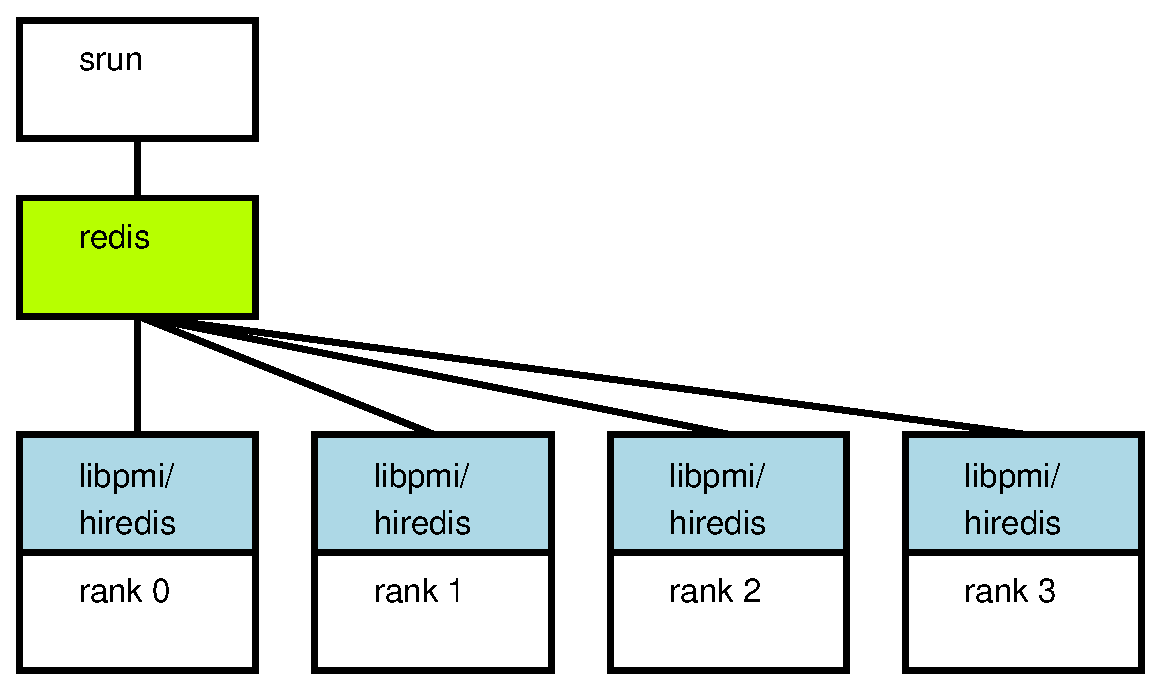
\includegraphics[scale=0.40]{redis-pmi.eps}
\caption{redis-pmi prototype architecture}
\label{fig:redispmi}
\end{figure}

Barriers are implemented as an atomic counter in redis using an embedded
Lua script.
Once all the MPI ranks have incremented the counter and blocked waiting
for a subscribed-to redis message, redis publishes a message indicating
that the barrier is complete.

Each MPI rank establishes two connections with redis, one for receiving
messages published by the barrier Lua function, and one for everything else.
Better scalability could be obtained by inserting a proxy layer (such as
{\em twemproxy}) between ranks and the redis server to reduce connection
overhead, by sharding to multiple servers, and by reimplementing barriers
using a reduction tree.

\subsection{Analysis of PMI API Usage by \mvapich2 and \openmpi}

Although a canonical PMIv1 header file is supplied by MPICH,
\slurm\ implements a superset of the canonical functions shown in
Table~\ref{tab:pmiv1}.  It is unclear where these functions are
standardized although some appear to have origins in the MPICH
SMPD process manager used on Windows, and some are documented in
the informal paper {\em Process Management in MPICH} distributed
with the MPICH source code.

\mvapich2\ 1.7, as built for TOSS 2.0 production, uses the canonical
PMIv1 interfaces indicated in the table.
Table~\ref{tab:mvapich} shows how it uses the KVS to launch a simple MPI
hello world program on shared memory.
Table~\ref{tab:mvapichpsm} shows the same on QLogic Infiniband, one task
per node.

\openmpi\ 1.6, as built for production does not use PMI;
however when configured {\tt --with-pmi --with-slurm} uses the 
PMI canoncal and extended interfaces indicated in Table~\ref{tab:pmiv1}.
Table~\ref{tab:openmpi} shows how it uses the KVS to launch a smple MPI
hello world program on shared memory.
\openmpi\ can be configured {\tt --with-cray-pmi-ext} which
activates a mixed use of PMIv2 and PMIv1; however this mode was not analyzed.

\begin{table}
\centering
\begin{tabular}{|p{4cm}|p{4cm}|p{4cm}|p{4cm}|}\hline
\textbf{proc 0} &       \textbf{proc 1} &   \textbf{proc 2} &    \textbf{proc 3}\\
\hline
put hostname[0] &     put hostname[1] &     put hostname[2] &     put hostname[3]\\
commit &              commit &              commit  &             commit\\
barrier &             barrier &             barrier &             barrier\\
\hline
get hostname[1] &     get hostname[0] &     get hostname[0] &     get hostname[0]\\
get hostname[2] &     get hostname[2] &     get hostname[1] &     get hostname[1]\\
get hostname[3] &     get hostname[3] &     get hostname[3] &     get hostname[2]\\
put sharedFilename[0] & & & \\
commit  & & &\\
barrier& barrier & barrier & barrier\\
\hline
 &                     get sharedFilename[0]&get sharedFilename[0]&get sharedFilename[0]\\
put P0-businesscard & put P1-businesscard & put P2-businesscard & put P3-businesscard\\
commit &              commit &              commit &              commit\\
barrier &             barrier &             barrier &             barrier\\
\hline
\end{tabular}
\caption{\mvapich2 PMI key-value store usage when launching a simple 
MPI hello world application on four procs using shared memory.
The shared memory file
is set up by rank 0 and communicated to the other tasks in {\tt sharedFilename}.
{\tt PN-businesscard} defines a unique {\em host:port} for each rank, e.g.
``{\tt description\#jimbo.chaos\$port\#39666\$ifname\#192.168.1.136\$}''}
\label{tab:mvapich}
\end{table}

\begin{table}
\centering
\begin{tabular}{|p{4cm}|p{4cm}|p{4cm}|p{4cm}|}\hline
\textbf{proc 0} &       \textbf{proc 1} &   \textbf{proc 2} &    \textbf{proc 3}\\
\hline
put hostname[0] &     put hostname[1] &     put hostname[2] &     put hostname[3]\\
commit &              commit &              commit  &             commit\\
barrier &             barrier &             barrier &             barrier\\
\hline
get hostname[1] &     get hostname[0] &     get hostname[0] &     get hostname[0]\\
get hostname[2] &     get hostname[2] &     get hostname[1] &     get hostname[1]\\
get hostname[3] &     get hostname[3] &     get hostname[3] &     get hostname[2]\\
barrier& barrier & barrier & barrier\\
\hline
put uuid\_0\_job1099867
  & put uuid\_1\_job1099867
  & put uuid\_2\_job1099867
  & put uuid\_3\_job1099867 \\
commit &              commit &              commit &              commit\\
barrier &             barrier &             barrier &             barrier\\
\hline
  & get uuid\_0\_job1099867
  & get uuid\_0\_job1099867
  & get uuid\_0\_job1099867 \\
barrier &             barrier &             barrier &             barrier\\
barrier &             barrier &             barrier &             barrier\\
barrier &             barrier &             barrier &             barrier\\
\hline
put pmi\_epidkey\_0
  & put pmi\_epidkey\_1
  & put pmi\_epidkey\_2
  & put pmi\_epidkey\_3\\
commit &              commit &              commit &              commit\\
barrier &             barrier &             barrier &             barrier\\
\hline
get pmi\_epidkey\_1
  & get pmi\_epidkey\_0
  & get pmi\_epidkey\_0
  & get pmi\_epidkey\_0\\
get pmi\_epidkey\_2
  & get pmi\_epidkey\_2
  & get pmi\_epidkey\_1
  & get pmi\_epidkey\_1\\
get pmi\_epidkey\_3
  & get pmi\_epidkey\_3
  & get pmi\_epidkey\_3
  & get pmi\_epidkey\_2\\
barrier &             barrier &             barrier &             barrier\\
\hline
\end{tabular}
\caption{\mvapich2 PMI key-value store usage when launching a simple 
MPI hello world application on four procs on infiniband (one proc per node).}
\label{tab:mvapichpsm}
\end{table}


\begin{table}
\centering
\begin{tabular}{|p{4cm}|p{4cm}|p{4cm}|p{4cm}|}\hline
\textbf{proc 0} &       \textbf{proc 1} &   \textbf{proc 2} &    \textbf{proc 3}\\
\hline
put [[0,1],0]-THD\_LEV
 & put [[0,1],1]-THD\_LEV
 & put [[0,1],2]-THD\_LEV
 & put [[0,1],3]-THD\_LEV\\
put [[0,1],0]-OMPI\_ARCH
 & put [[0,1],1]-OMPI\_ARCH
 & put [[0,1],2]-OMPI\_ARCH
 & put [[0,1],3]-OMPI\_ARCH\\
put [[0,1],0]-btl.sctp.1.6
 &  put [[0,1],1]-btl.sctp.1.6
 &  put [[0,1],2]-btl.sctp.1.6
 &  put [[0,1],3]-btl.sctp.1.6\\
put [[0,1],0]-btl.tcp.1.6
 &  put [[0,1],1]-btl.tcp.1.6
 &  put [[0,1],2]-btl.tcp.1.6
 &  put [[0,1],3]-btl.tcp.1.6\\
put [[0,1],0]-HOSTNAME
 &  put [[0,1],1]-HOSTNAME
 &  put [[0,1],2]-HOSTNAME
 &  put [[0,1],3]-HOSTNAME\\
put [[0,1],0]-RMLURI
 &  put [[0,1],1]-RMLURI
 &  put [[0,1],2]-RMLURI
 &  put [[0,1],3]-RMLURI\\
put [[0,1],0]-LOCRANK
 &  put [[0,1],1]-LOCRANK
 &  put [[0,1],2]-LOCRANK
 &  put [[0,1],3]-LOCRANK\\
put [[0,1],0]-NODERANK
 &  put [[0,1],1]-NODERANK
 &  put [[0,1],2]-NODERANK
 &  put [[0,1],3]-NODERANK\\
commit & commit & commit & commit \\  
barrier& barrier& barrier& barrier\\  
\hline
get [[0,1],1]-RMLURI
 &  get [[0,1],0]-RMLURI
 &  get [[0,1],0]-RMLURI
 &  get [[0,1],0]-RMLURI\\
get [[0,1],1]-HOSTNAME
 &  get [[0,1],0]-HOSTNAME
 &  get [[0,1],0]-HOSTNAME
 &  get [[0,1],0]-HOSTNAME\\
get [[0,1],1]-LOCRANK
 &  get [[0,1],0]-LOCRANK
 &  get [[0,1],0]-LOCRANK
 &  get [[0,1],0]-LOCRANK\\
get [[0,1],1]-NODERANK
 &  get [[0,1],0]-NODERANK
 &  get [[0,1],0]-NODERANK
 &  get [[0,1],0]-NODERANK\\
\hline
get [[0,1],2]-RMLURI
 &  get [[0,1],2]-RMLURI
 &  get [[0,1],1]-RMLURI
 &  get [[0,1],1]-RMLURI\\
get [[0,1],2]-HOSTNAME
 &  get [[0,1],2]-HOSTNAME
 &  get [[0,1],1]-HOSTNAME
 &  get [[0,1],1]-HOSTNAME\\
get [[0,1],2]-LOCRANK
 &  get [[0,1],2]-LOCRANK
 &  get [[0,1],1]-LOCRANK
 &  get [[0,1],1]-LOCRANK\\
get [[0,1],2]-NODERANK
 &  get [[0,1],2]-NODERANK
 &  get [[0,1],1]-NODERANK
 &  get [[0,1],1]-NODERANK\\
\hline
get [[0,1],3]-RMLURI
 &  get [[0,1],3]-RMLURI
 &  get [[0,1],3]-RMLURI
 &  get [[0,1],2]-RMLURI\\
get [[0,1],3]-HOSTNAME
 &  get [[0,1],3]-HOSTNAME
 &  get [[0,1],3]-HOSTNAME
 &  get [[0,1],2]-HOSTNAME\\
get [[0,1],3]-LOCRANK
 &  get [[0,1],3]-LOCRANK
 &  get [[0,1],3]-LOCRANK
 &  get [[0,1],2]-LOCRANK\\
get [[0,1],3]-NODERANK
 &  get [[0,1],3]-NODERANK
 &  get [[0,1],3]-NODERANK
 &  get [[0,1],2]-NODERANK\\
\hline
get [[0,1],1]-OMPI\_ARCH
 &  get [[0,1],0]-OMPI\_ARCH
 &  get [[0,1],0]-OMPI\_ARCH
 &  get [[0,1],0]-OMPI\_ARCH\\
get [[0,1],2]-OMPI\_ARCH
 &  get [[0,1],2]-OMPI\_ARCH
 &  get [[0,1],1]-OMPI\_ARCH
 &  get [[0,1],1]-OMPI\_ARCH\\
get [[0,1],3]-OMPI\_ARCH
 &  get [[0,1],3]-OMPI\_ARCH
 &  get [[0,1],3]-OMPI\_ARCH
 &  get [[0,1],2]-OMPI\_ARCH\\
\hline
get [[0,1],1]-btl.tcp.1.6
 &  get [[0,1],0]-btl.tcp.1.6
 &  get [[0,1],0]-btl.tcp.1.6
 &  get [[0,1],0]-btl.tcp.1.6\\
get [[0,1],2]-btl.tcp.1.6
 &  get [[0,1],2]-btl.tcp.1.6
 &  get [[0,1],1]-btl.tcp.1.6
 &  get [[0,1],1]-btl.tcp.1.6\\
get [[0,1],3]-btl.tcp.1.6
 &  get [[0,1],3]-btl.tcp.1.6
 &  get [[0,1],3]-btl.tcp.1.6
 &  get [[0,1],2]-btl.tcp.1.6\\
\hline
get [[0,1],0]-btl.tcp.1.6
 &  get [[0,1],1]-btl.tcp.1.6
 &  get [[0,1],2]-btl.tcp.1.6
 &  get [[0,1],3]-btl.tcp.1.6\\
get [[0,1],1]-btl.tcp.1.6
 &  get [[0,1],0]-btl.tcp.1.6
 &  get [[0,1],0]-btl.tcp.1.6
 &  get [[0,1],0]-btl.tcp.1.6\\
get [[0,1],2]-btl.tcp.1.6
 &  get [[0,1],2]-btl.tcp.1.6
 &  get [[0,1],1]-btl.tcp.1.6
 &  get [[0,1],1]-btl.tcp.1.6\\
get [[0,1],3]-btl.tcp.1.6
 &  get [[0,1],3]-btl.tcp.1.6
 &  get [[0,1],3]-btl.tcp.1.6
 &  get [[0,1],2]-btl.tcp.1.6\\
\hline
get [[0,1],1]-btl.sctp.1.6
 &  get [[0,1],0]-btl.sctp.1.6
 &  get [[0,1],0]-btl.sctp.1.6
 &  get [[0,1],0]-btl.sctp.1.6\\
get [[0,1],2]-btl.sctp.1.6
 &  get [[0,1],2]-btl.sctp.1.6
 &  get [[0,1],1]-btl.sctp.1.6
 &  get [[0,1],1]-btl.sctp.1.6\\
get [[0,1],3]-btl.sctp.1.6
 &  get [[0,1],3]-btl.sctp.1.6
 &  get [[0,1],3]-btl.sctp.1.6
 &  get [[0,1],2]-btl.sctp.1.6\\
get [[0,1],0]-btl.sctp.1.6
 &  get [[0,1],1]-btl.sctp.1.6
 &  get [[0,1],2]-btl.sctp.1.6
 &  get [[0,1],3]-btl.sctp.1.6\\
commit & commit & commit & commit \\  
barrier& barrier& barrier& barrier\\  
\hline
get [[0,1],0]-THD\_LEV
 &  get [[0,1],0]-THD\_LEV
 &  get [[0,1],0]-THD\_LEV
 &  get [[0,1],0]-THD\_LEV\\
get [[0,1],1]-THD\_LEV
 &  get [[0,1],1]-THD\_LEV
 &  get [[0,1],1]-THD\_LEV
 &  get [[0,1],1]-THD\_LEV\\
get [[0,1],2]-THD\_LEV
 &  get [[0,1],2]-THD\_LEV
 &  get [[0,1],2]-THD\_LEV
 &  get [[0,1],2]-THD\_LEV\\
get [[0,1],3]-THD\_LEV
 &  get [[0,1],3]-THD\_LEV
 &  get [[0,1],3]-THD\_LEV
 &  get [[0,1],3]-THD\_LEV\\
\hline
\end{tabular}
\caption{openmpi PMI key-value store usage when launching a simple 
MPI hello world application on four procs using shared memory.
Abbreviations used: MPI\_THREAD\_LEVEL $=$ THD\_LEV; LOCALRANK $=$ LOCRANK.
}
\label{tab:openmpi}
\end{table}

\begin{table}
\centering
\begin{tabular}{|p{5cm}|p{3.5cm}|p{3cm}|p{3cm}|}\hline
\textbf{Function} & \textbf{\mvapich2-1.7 shmem}
		  & \textbf{\mvapich2-1.7 psm}
		  & \textbf{\openmpi-1.6 shmem}\\
\hline
\multicolumn{4}{|c|}{\textbf{Canonical PMI-1 Functions}}\\
\hline
{\tt  PMI\_Init} & $n$ & $n$ & $n$\\
\hline
{\tt  PMI\_Initialized} & $-$ & $-$ & $n$\\
\hline
{\tt  PMI\_Finalize} & $n$ & $n$ & $-$\\
\hline
{\tt  PMI\_Get\_size} & $n$ & $n$ & $-$\\
\hline
{\tt  PMI\_Get\_rank} & $n$ & $n$ & $n$\\
\hline
{\tt  PMI\_Get\_universe\_size} & $-$ & $-$ & $n$\\
\hline
{\tt  PMI\_Get\_appnum} & $n$ & $n$ & $n$\\
\hline
{\tt  PMI\_Publish\_name} & $-$ & $-$ & $-$\\
\hline
{\tt  PMI\_Unpublish\_name} & $-$ & $-$ & $-$\\
\hline
{\tt  PMI\_Lookup\_name} & $-$ & $-$ & $-$\\
\hline
{\tt  PMI\_Barrier} & $3n$ & $7n$ & $3n$ \\
\hline
{\tt  PMI\_Abort} & $-$ & $-$ & $-$\\
\hline
{\tt  PMI\_KVS\_Get\_my\_name} & $2n$ & $2n$ & $n$\\
\hline
{\tt  PMI\_KVS\_Get\_name\_length\_max} & $2n$ & $2n$ & $n$\\
\hline
{\tt  PMI\_KVS\_Get\_key\_length\_max} & $3n$ & $5n$ & $n$\\
\hline
{\tt  PMI\_KVS\_Get\_value\_length\_max} & $3n$ & $3n$ & $n$\\
\hline
{\tt  PMI\_KVS\_Put} & $2n + 1$ & $3n$ & $8n$\\
\hline
{\tt  PMI\_KVS\_Commit} & $2n + 1$ & $3n$ & $n$\\
\hline
{\tt  PMI\_KVS\_Get} & $n(n -1) + n$ & $(2n + 1)(n -1)$ & $3n^2 + 6n(n - 1)$ \\
\hline
{\tt  PMI\_Spawn\_multiple} & $-$ & $-$ & $-$ \\
\hline
\multicolumn{4}{|c|}{\textbf{Extended PMI-1 Functions}}\\
\hline
{\tt  PMI\_Get\_id} & $-$ & $-$ & $-$ \\
\hline
{\tt  PMI\_Get\_kvs\_domain\_id} & $-$ & $-$ & $n$ \\
\hline
{\tt  PMI\_Get\_id\_length\_max} & $-$ & $-$ & $n$ \\
\hline
{\tt  PMI\_Get\_clique\_size} & $-$ & $-$ & $n$ \\
\hline
{\tt  PMI\_Get\_clique\_ranks} & $-$ & $-$ & $n$ \\
\hline
{\tt  PMI\_KVS\_Create} & $-$ & $-$ & $-$ \\
\hline
{\tt  PMI\_KVS\_Create} & $-$ & $-$ & $-$ \\
\hline
{\tt  PMI\_KVS\_Destroy} & $-$ & $-$ & $-$ \\
\hline
{\tt  PMI\_KVS\_Iter\_first} & $-$ & $-$ & $-$ \\
\hline
{\tt  PMI\_KVS\_Iter\_next} & $-$ & $-$ & $-$ \\
\hline
{\tt  PMI\_Parse\_option} & $-$ & $-$ & $-$ \\
\hline
{\tt  PMI\_Args\_to\_keyval} & $-$ & $-$ & $-$ \\
\hline
{\tt  PMI\_Free\_keyvals} & $-$ & $-$ & $-$ \\
\hline
{\tt  PMI\_Get\_options} & $-$ & $-$ & $-$\\
\hline
\end{tabular}
\caption{PMI functions implemented by \slurm.
Their usage in support of launching a simple MPI hello world program
is shown for \mpich2 (shmem and psm) and \openmpi.
The column entries list the total number of calls,
expressed in terms of $n$, the number of MPI ranks.}
\label{tab:pmiv1}
\end{table}


%\bibliographystyle{abbrv}
%\bibliography{../bib/project,../bib/rfc}

\end{document}
